\input{../../template.ltx}

\usepackage{multicol}
\usepackage{tikz}
\usetikzlibrary{arrows}

\begin{document}

\osuetitle{3}

\section*{3-Coloring}
\label{sec:intro}

Implement an algorithm which makes a graph 3-colorable
by removing the least edges possible.
A graph is 3-colorable if it is possible to assign one of 3 colors to each vertex,
such that no two connected vertices share the same color.

For instance, consider the following graph:

\begin{center}
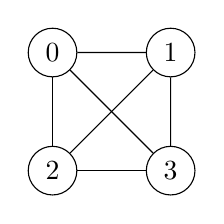
\begin{tikzpicture}[scale=1.5,>=triangle 60]
    \node[shape=circle,draw=black] (0) at (0,1) {0};
    \node[shape=circle,draw=black] (1) at (1,1) {1};
    \node[shape=circle,draw=black] (2) at (0,0) {2};
    \node[shape=circle,draw=black] (3) at (1,0) {3};
    \path[-](0) edge node {} (1);
    \path[-](0) edge node {} (2);
    \path[-](0) edge node {} (3);
    \path[-](1) edge node {} (2);
    \path[-](1) edge node {} (3);
    \path[-](2) edge node {} (3);
\end{tikzpicture}
\end{center}

This graph is not 3-colorable;
however it can be made 3-colorable by removing the edge $(\,0,1\,)$:

\begin{center}
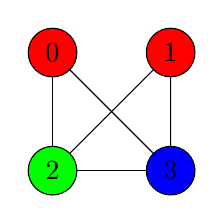
\begin{tikzpicture}[scale=1.5,>=triangle 60]
    \node[shape=circle,draw=black,fill=red] (0) at (0,1) {0};
    \node[shape=circle,draw=black,fill=red] (1) at (1,1) {1};
    \node[shape=circle,draw=black,fill=green] (2) at (0,0) {2};
    \node[shape=circle,draw=black,fill=blue] (3) at (1,0) {3};
    \path[-](0) edge node {} (2);
    \path[-](0) edge node {} (3);
    \path[-](1) edge node {} (2);
    \path[-](1) edge node {} (3);
    \path[-](2) edge node {} (3);
\end{tikzpicture}
\end{center}

Thus $\{\;(\,0,1\,)\;\}$ is a minimal set of edges
which must be removed to make this graph 3-colorable.
Note that there are other such sets of equal length,
for instance $\{\;(\,0,2\,)\;\}$, $\{\;(\,0,3\,)\;\}$ or $\{\;(\,2,3\,)\;\}$.

The problem of deciding whether a graph is 3-colorable is NP-complete
and the same is true for the problem of finding a minimal set of edges
to make a graph 3-colorable.
Therefore an exact solution becomes infeasible for moderately large graph sizes.
However, a randomized algorithm can be used to find a good approximation,
i.e. to find a set of edges which is close to minimal.
\footnote{
You can read more about the complexity of the 3-colorability problem
and about Monte Carlo randomized algorithms in general on Wikipedia:\\
\url{https://en.wikipedia.org/wiki/Graph_coloring}\\
\url{https://en.wikipedia.org/wiki/Monte_Carlo_algorithm}\\
}

A simple randomized algorithm for this problem generates a set of edges
which must be removed to make a given graph 3-colorable
by executing following steps:

\begin{itemize}
\item Generate a random (not necessarily valid) 3-coloring of the graph,
i.e. randomly assign one of 3 colors to each vertex of the graph.

\item Select all edges $(\,u,v\,)$ for which
the color of $u$ is identical to the color of $v$.
These edges need to be removed to make the graph 3-colorable.

\emph{Proof:}
Once these edges have been removed,
the previously generated 3-coloring becomes valid.
Thus removing these edges makes the graph 3-colorable.
\end{itemize}

These steps are executed repeatedly and the smallest set of edges so far is retained.

Although it might seem surprising given its simplicity,
this algorithm has an expected runtime which is polynomial in the size of the graph
and thus is on average much faster than an algorithm which tries to find an exact solution.

\clearpage
\subsection*{Instructions}

In order to further reduce the runtime of this algorithm,
multiple processes generate the random sets of edges in parallel
and report their results to a supervisor process,
which remembers the set with the least edges.

Write two programs: a \textbf{generator program} and a \textbf{supervisor program}.
\textbf{Multiple generator processes} generate random solutions to the problem
and report their solutions to \textbf{one supervisor process}.
The supervisor process remembers the best solution so far.
The processes communicate with eachother by means of a circular buffer,
which is implemented using shared semaphores and a shared memory.

\subsubsection*{Supervisor}

The supervisor sets up the shared memory and the semaphores
and initializes the circular buffer
required for the communication with the generators.
It then waits for the generators to write solutions to the circular buffer
and reads these solutions, remembering the best solution so far.

The supervisor program takes no arguments.

Once initialization is complete,
the supervisor reads the solutions from the circular buffer
and remembers the best solution so far, i.e. the solution with the least edges.
Every time a better solution than the previous best solution is found,
the supervisor writes the new solution to standard output.
If a generator writes a solution with 0 edges to the circular buffer,
then the graph is acyclic and the supervisor aborts the algorithm.
Otherwise the supervisor keeps reading results from the circular buffer
until it receives a \texttt{SIGINT} or a \texttt{SIGTERM} signal.

Before terminating, the supervisor notifies all generators
that they should terminate as well.
This can be done by setting a variable in the shared memory,
which is checked by the generator processes before writing to the buffer.
The supervisor then unlinks all shared resources and exits.

\subsubsection*{Generator}

The generator program takes a graph as input.
The program repeatedly generates a random solution to the problem as described on the first page
and writes its result to the circular buffer.
It repeats this procedure until it is notified by the supervisor to terminate.

The generator program takes as arguments the set of edges of the graph:

\begin{verbatim}
    SYNOPSIS
        generator EDGE1...
    EXAMPLE
        generator 0-1 0-2 0-3 1-2 1-3 2-3
\end{verbatim}

Each positional argument is one edge; at least one edge must be given.
An edge is specified by a string,
with the indices of the two nodes it connects separated by a \texttt{-}.
Note that the number of nodes of the graph is implicitly provided
through the indices in the edges.
In the example above the generator program is called with the graph shown on the top of the first page.

The generator uses the algorithm described on the first page
to generate random sets of edges which must be removed to make the given graph 3-colorable.
It writes these edge sets to the circular buffer, one at a time;
therefore a set of edges is a single element of the circular buffer.
The generator may produce debug output,
describing the edge sets which it writes to the circular buffer.

\clearpage
\subsubsection*{Circular Buffer}

The generators report their solutions to the supervisor by means of a circular buffer.
The generators write their solutions to the write end of the circular buffer
and the supervisor reads them from the read end.

A circular buffer is a common data structure which uses a single fixed-size buffer
to implement a queue (i.e. a FIFO buffer).
A circular buffer is essentially \textbf{an array of the elements} you want to pass through.
Elements are written successively to the array
and once the end of the array is reached, writing restarts from the beginning.
Similarly, elements are also read successively from the array,
restarting from the beginning upon reaching the end,
thus reading the elements in the exact same order they have been written.
\footnote{
Visualizations of circular buffers can be found on Wikipedia:\\
\url{https://en.wikipedia.org/wiki/Circular_buffer}\\
}

Implement your circular buffer such that \textbf{reading and writing} to the buffer
can happen \textbf{simultaneously}.
Some synchronization is required
in order to avoid overwriting data which has not been read yet
and also to avoid trying to read from locations which have not been written yet.
This is achieved using two semaphores:
\textbf{one semaphore tracking the free space} in the circular buffer
and \textbf{one semaphore tracking the used space}.
The value of the free space semaphore corresponds to the amount of free space in the buffer array;
it is initialized to the size of the buffer, since initially the circular buffer is empty.
The value of the used space semaphore corresponds to the amount of used space in the buffer array;
it is initialized to 0.

Upon \textbf{writing to the circular buffer}, the free space semaphore is decremented;
if the buffer is currently full and there is no free space to write to,
this intentionally blocks the write until space becomes available.
After the write is complete, the used space semaphore is incremented,
since the buffer now holds one more element which can be read.

Upon \textbf{reading from the circular buffer}, the used space semaphore is decremented;
if the buffer is currently empty and there is no data to be read,
this intentionally blocks the read until data becomes available.
After the read is complete, the free space semaphore is incremented,
since the position occupied by the element which has been read just has been freed up.

Since multiple generators write to the circular buffer,
an additional semaphore will be required
to guarantee a \textbf{mutually exclusive access to the write end} of the circular buffer.

\subsection*{Hints}
\begin{itemize}
\item Store the graph in a way which is suitable for the implementation of the randomized algorithm.

\item Think of a suitable structure to store a set of edges.
Choose a limit on the maximum number of edges which it can contain.
Since we are looking for small solutions,
the generator can discard any solutions which contain too much edges
instead of writing them to the circular buffer.
You may choose a limit as low as 8 edges.

\item Select a reasonable size for the circular buffer.
If the size is too small,
then the generators will spend a lot of time waiting for free space to become available.
If the size is too large,
the circular buffer is wasting resources.
The size of the shared memory should not exceed 4~KiB.

\end{itemize}

\clearpage
\subsection*{Examples}
\setlength{\columnsep}{-20mm}

\begin{multicols}{2}
\subsubsection*{Simple 3-colorable graph}

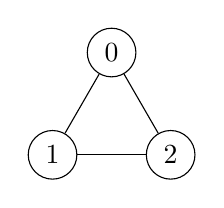
\begin{tikzpicture}[scale=1.5,>=triangle 60]
    \node[shape=circle,draw=black] (0) at (0.5,0.866) {0};
    \node[shape=circle,draw=black] (1) at (0,0) {1};
    \node[shape=circle,draw=black] (2) at (1,0) {2};
    \path[-](0) edge node {} (1);
    \path[-](1) edge node {} (2);
    \path[-](2) edge node {} (0);
\end{tikzpicture}

This graph is already 3-colorable.

\vfill

~

\columnbreak

\textbf{Invocation of the supervisor:}
\vspace{-5mm}
\begin{verbatim}
$ ./supervisor
[./supervisor] Solution with 1 edges: 0-2
[./supervisor] The graph is 3-colorable!
\end{verbatim}

\textbf{Invocation of one generator:}
\vspace{-5mm}
\begin{verbatim}
$ ./generator 0-1 0-2 1-2
\end{verbatim}

\textbf{Invocation of 10 generators in parallel:}
\vspace{-5mm}
\begin{verbatim}
$ for i in {1..10}; do (./generator 0-1 0-2 1-2 &); done
\end{verbatim}
\end{multicols}

\vspace{7mm}
\begin{multicols}{2}
\subsubsection*{Graph from the first page}

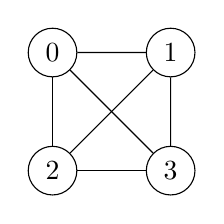
\begin{tikzpicture}[scale=1.5,>=triangle 60]
    \node[shape=circle,draw=black] (0) at (0,1) {0};
    \node[shape=circle,draw=black] (1) at (1,1) {1};
    \node[shape=circle,draw=black] (2) at (0,0) {2};
    \node[shape=circle,draw=black] (3) at (1,0) {3};
    \path[-](0) edge node {} (1);
    \path[-](0) edge node {} (2);
    \path[-](0) edge node {} (3);
    \path[-](1) edge node {} (2);
    \path[-](1) edge node {} (3);
    \path[-](2) edge node {} (3);
\end{tikzpicture}

Removing one edge is sufficient to\\
make this graph 3-colorable, as seen\\
on the first page.

\columnbreak

\textbf{Invocation of the supervisor:}
\vspace{-5mm}
\begin{verbatim}
$ ./supervisor
[./supervisor] Solution with 2 edges: 0-3 1-2
[./supervisor] Solution with 1 edges: 0-1
\end{verbatim}

\textbf{Invocation of the generator:}
\vspace{-5mm}
\begin{verbatim}
$ ./generator 0-1 0-2 0-3 1-2 1-3 2-3
\end{verbatim}
\end{multicols}

\vspace{7mm}
\begin{multicols}{2}
\subsubsection*{More complex graph}

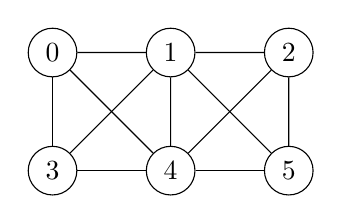
\begin{tikzpicture}[scale=1.5,>=triangle 60]
    \node[shape=circle,draw=black] (0) at (0,1) {0};
    \node[shape=circle,draw=black] (1) at (1,1) {1};
    \node[shape=circle,draw=black] (2) at (2,1) {2};
    \node[shape=circle,draw=black] (3) at (0,0) {3};
    \node[shape=circle,draw=black] (4) at (1,0) {4};
    \node[shape=circle,draw=black] (5) at (2,0) {5};
    \path[-](0) edge node {} (1);
    \path[-](0) edge node {} (3);
    \path[-](0) edge node {} (4);
    \path[-](1) edge node {} (2);
    \path[-](1) edge node {} (3);
    \path[-](1) edge node {} (4);
    \path[-](1) edge node {} (5);
    \path[-](2) edge node {} (4);
    \path[-](2) edge node {} (5);
    \path[-](3) edge node {} (4);
    \path[-](4) edge node {} (5);
\end{tikzpicture}

\vfill

This graph can again be made\\
3-colorable by removing a single\\
edge.

\columnbreak

\textbf{Invocation of the supervisor:}
\vspace{-5mm}
\begin{verbatim}
$ ./supervisor
[./supervisor] Solution with 4 edges: 0-3 0-4 1-2 3-4
[./supervisor] Solution with 3 edges: 0-4 1-2 4-5
[./supervisor] Solution with 2 edges: 1-3 1-5
[./supervisor] Solution with 1 edges: 1-4
\end{verbatim}

\textbf{Invocation of the generator:}
\vspace{-5mm}
\begin{verbatim}
$ ./generator 0-1 0-3 0-4 1-2 1-3 1-4 1-5 2-4 2-5 3-4 4-5
\end{verbatim}
\end{multicols}

\vspace{5mm}
If you want to test your implementation with a challenging graph, try this one
\footnote{
Source: Graph \#3349 from the House of Graphs:
\url{https://hog.grinvin.org/ViewGraphInfo.action?id=3349}
}:

\texttt{0-1 0-2 0-3 1-28 1-29 2-30 2-31 3-32 3-33 4-6 4-14 4-16 5-7 5-15 5-17 6-7 6-18 7-19\\
8-9 8-12 8-23 9-13 9-22 10-15 10-19 10-25 11-14 11-18 11-24 12-17 12-27 13-16 13-26\\
14-23 15-22 16-21 17-20 18-21 19-20 20-31 21-30 22-33 23-32 24-27 24-29 25-26 25-29\\
26-28 27-28 30-33 31-32}

Note: This graph is 3-colorable,
therefore one of your generators should eventually come up with a solution with 0 edges.

\osueguidelinesthree

\end{document}
